\RequirePackage[l2tabu,orthodox]{nag}

% TODO: decide if one-sided/two-sided
%\documentclass[headsepline,footsepline,footinclude=false,fontsize=11pt,paper=a4,listof=totoc,bibliography=totoc,BCOR=12mm,DIV=12]{scrbook} % two-sided % original source stated: BCOR=12mm,DIV=12
\documentclass[headsepline,footsepline,footinclude=false,oneside,fontsize=11pt,paper=a4,listof=totoc,bibliography=totoc,DIV=12,fleqn]{scrbook} % one-sided
\setlength\mathindent{0pt} %=======added by Qinglong: 'fleqn' in the document class and this command make all equations aligned to the left.

\usepackage{mathptmx}
\usepackage[T1]{fontenc}
% TODO: change citation style in settings
\usepackage{array} %for table values centering, can delete
%\usepackage{graphicx} %for pictures in same line, can delete
\usepackage[titletoc]{appendix} %for appendix setting, can delete
\newcolumntype{P}[1]{>{\centering\arraybackslash}p{#1}} %for table values centering, can delete if doesn't work
\usepackage{afterpage} %for blank page after appendix
\newcommand\blankpage{
    \null
    \thispagestyle{empty}
    \addtocounter{page}{-1}
    \newpage
    }
\usepackage{listings} %for python in appendix
\usepackage{xcolor} %for proper format of python code



\definecolor{codegreen}{rgb}{0,0.6,0}
\definecolor{codegray}{rgb}{0.5,0.5,0.5}
\definecolor{codepurple}{rgb}{0.58,0,0.82}
\definecolor{backcolour}{rgb}{0.95,0.95,0.92}
\lstdefinestyle{mystyle}{
    backgroundcolor=\color{backcolour},   
    commentstyle=\color{codegreen},
    keywordstyle=\color{magenta},
    numberstyle=\tiny\color{codegray},
    stringstyle=\color{codepurple},
    basicstyle=\ttfamily\footnotesize,
    breakatwhitespace=false,         
    breaklines=true,                 
    captionpos=b,                    
    keepspaces=true,                 
    numbers=left,                    
    numbersep=5pt,                  
    showspaces=false,                
    showstringspaces=false,
    showtabs=false,                  
    tabsize=2
}

\lstset{style=mystyle}


\PassOptionsToPackage{table,svgnames,dvipsnames}{xcolor}

\usepackage[utf8]{inputenc}
\usepackage[T1]{fontenc}
\usepackage[sc]{mathpazo}
\usepackage[ngerman,english]{babel} % english is the same as american or USenglish
\usepackage[autostyle]{csquotes}
%==================================


% \usepackage[authordate,bibencoding=auto,strict,backend=biber,natbib]{biblatex-chicago}
% \addbibresource{bibliography.bib}
%==============================
\usepackage{graphicx}
\usepackage{scrhack} % necessary for listings package
\usepackage{listings}
\usepackage{lstautogobble}
\usepackage{tikz}
\usepackage{pgfplots}
\usepackage{pgfplotstable}
\usepackage{booktabs} % for better looking table creations, but bad with vertical lines by design (package creator despises vertical lines)
\usepackage[final]{microtype}
\usepackage{caption}
\usepackage[hidelinks]{hyperref} % hidelinks removes colored boxes around references and links
\usepackage{ifthen} % for comparison of the current language and changing of the thesis layout
\usepackage{pdftexcmds} % string compare to work with all engines
\usepackage{paralist} % for condensed enumerations or lists
\usepackage{subfig} % for having figures side by side
\usepackage{siunitx} % for physical accurate units and other numerical presentations
\usepackage{multirow} % makes it possible to have bigger cells over multiple rows in a table
\usepackage{array} % different options for table cell orientation
\usepackage{makecell} % allows nice manual configuration of cells with linebreaks in \thead and \makecell with alignments
\usepackage{pdfpages} % for including multiple pages of pdfs
\usepackage{adjustbox} % can center content wider than the \textwidth
\usepackage{tablefootnote} % for footnotes in tables as \tablefootnote
\usepackage{threeparttable} % another way to add footnotes as \tablenotes with \item [x] <your footnote> after setting \tnote{x} 


% https://tex.stackexchange.com/questions/42619/x-mark-to-match-checkmark
\usepackage{amssymb}% http://ctan.org/pkg/amssymb
\usepackage{pifont}% http://ctan.org/pkg/pifont
\newcommand{\cmark}{\ding{51}}%
\newcommand{\xmark}{\ding{55}}%


\usepackage[acronym,xindy,toc]{glossaries} % TODO: include "acronym" if glossary and acronym should be separated
\makeglossaries
% \loadglsentries{pages/glossary.tex} % important update for glossaries, before document


%\bibliography{bibliography}

\setkomafont{disposition}{\normalfont\bfseries} % use serif font for headings
\linespread{1.05} % adjust line spread for mathpazo font

% Add table of contents to PDF bookmarks
\BeforeTOCHead[toc]{{\cleardoublepage\pdfbookmark[0]{\contentsname}{toc}}}

% Define TUM corporate design colors
% Taken from http://portal.mytum.de/corporatedesign/index_print/vorlagen/index_farben
\definecolor{TUMBlue}{HTML}{0065BD}
\definecolor{TUMSecondaryBlue}{HTML}{005293}
\definecolor{TUMSecondaryBlue2}{HTML}{003359}
\definecolor{TUMBlack}{HTML}{000000}
\definecolor{TUMWhite}{HTML}{FFFFFF}
\definecolor{TUMDarkGray}{HTML}{333333}
\definecolor{TUMGray}{HTML}{808080}
\definecolor{TUMLightGray}{HTML}{CCCCC6}
\definecolor{TUMAccentGray}{HTML}{DAD7CB}
\definecolor{TUMAccentOrange}{HTML}{E37222}
\definecolor{TUMAccentGreen}{HTML}{A2AD00}
\definecolor{TUMAccentLightBlue}{HTML}{98C6EA}
\definecolor{TUMAccentBlue}{HTML}{64A0C8}

% Settings for pgfplots
\pgfplotsset{compat=newest}
\pgfplotsset{
  % For available color names, see http://www.latextemplates.com/svgnames-colors
  cycle list={TUMBlue\\TUMAccentOrange\\TUMAccentGreen\\TUMSecondaryBlue2\\TUMDarkGray\\},
}

% Settings for lstlistings

% Use this for basic highlighting
\lstset{%
  basicstyle=\ttfamily,
  columns=fullflexible,
  autogobble,
  keywordstyle=\bfseries\color{TUMBlue},
  stringstyle=\color{TUMAccentGreen}
}

% use this for C# highlighting
% %\setmonofont{Consolas} %to be used with XeLaTeX or LuaLaTeX
% \definecolor{bluekeywords}{rgb}{0,0,1}
% \definecolor{greencomments}{rgb}{0,0.5,0}
% \definecolor{redstrings}{rgb}{0.64,0.08,0.08}
% \definecolor{xmlcomments}{rgb}{0.5,0.5,0.5}
% \definecolor{types}{rgb}{0.17,0.57,0.68}

% \lstset{language=[Sharp]C,
% captionpos=b,
% %numbers=left, % numbering
% %numberstyle=\tiny, % small row numbers
% frame=lines, % above and underneath of listings is a line
% showspaces=false,
% showtabs=false,
% breaklines=true,
% showstringspaces=false,
% breakatwhitespace=true,
% escapeinside={(*@}{@*)},
% commentstyle=\color{greencomments},
% morekeywords={partial, var, value, get, set},
% keywordstyle=\color{bluekeywords},
% stringstyle=\color{redstrings},
% basicstyle=\ttfamily\small,
% }

% Settings for search order of pictures
\graphicspath{
    {logos/}
    {figures/}
}

% Set up hyphenation rules for the language package when mistakes happen
\babelhyphenation[english]{
an-oth-er
ex-am-ple
}

% Decide between
%\newcommand{\todo}[1]{\textbf{\textsc{\textcolor{TUMAccentOrange}{(TODO: #1)}}}} % for one paragraph, otherwise error!
%\newcommand{\done}[1]{\textit{\textsc{\textcolor{TUMAccentBlue}{(Done: #1)}}}} % for one paragraph, otherwise error!
% and
\newcommand{\todo}[1]{{\bfseries{\scshape{\color{TUMAccentOrange}[(TODO: #1)]}}}} % for multiple paragraphs
\newcommand{\done}[1]{{\itshape{\scshape{\color{TUMAccentBlue}[(Done: #1)]}}}} % for multiple paragraphs
% for error handling of intended behavior in your latex documents.

\newcommand{\tabitem}{~~\llap{\textbullet}~~}

\newcolumntype{P}[1]{>{\centering\arraybackslash}p{#1}} % for horizontal alignment with limited column width
\newcolumntype{M}[1]{>{\centering\arraybackslash}m{#1}} % for horizontal and vertical alignment with limited column width
\newcolumntype{L}[1]{>{\raggedright\arraybackslash}m{#1}} % for vertical alignment left with limited column width
\newcolumntype{R}[1]{>{\raggedleft\arraybackslash}m{#1}} % for vertical alignment right with limited column width
%===============added by Qinglong
\usepackage{cleveref}
\interfootnotelinepenalty=10000 % avoid long footnotes goes to the next page. 
\usepackage{algpseudocode}
\usepackage{cases}
\usepackage{tablefootnote}
%%%%%%
\usepackage[absolute]{textpos}
\usepackage{calc} % Berechnungen
\usepackage{tabto} % Tabulatoren
%\usepackage{parskip}
%%%%%%%

\newtheorem{assumption}{Assumption}[chapter] % for proofs and theorems
\newtheorem{prerequisite}{Prerequisite}[chapter]
%===============
\newcommand{\SeitenrandOben}{43.5mm}
\newcommand{\SeitenrandRechts}{20mm}
\newcommand{\SeitenrandLinks}{20mm}
\newcommand{\SeitenrandUnten}{10mm}

\newcommand{\UniversitaetLogoBreite}{19mm}
\newcommand{\UniversitaetLogoHoehe}{1cm}

\usepackage[
backend=biber,
style=apa,
sorting=anyt,
natbib
]{biblatex}\addbibresource{bibliography.bib}

\usepackage{color, colortbl}
\definecolor{Gray}{gray}{0.9}

\usepackage[ruled,vlined]{algorithm2e}
\DontPrintSemicolon 

\usepackage{float}

% TODO: change thesis information
\newcommand*{\getModule}{MA 05 Global Trends and Technology Assessment}
\newcommand*{\getUniversity}{Hochschule Koblenz - RheinAhrCampus}
%\newcommand*{\getFaculty}{}
%\newcommand*{\getOrganization}{Siemens Mobility}
\newcommand*{\getChair}{Wirtschafts- und Sozialwissenschaften}
\newcommand*{\getTitle}{Economic Trends: Social Inequality}
%\newcommand*{\getTitleGer}{Titel der Abschlussarbeit}
\newcommand*{\getAuthor}{Ashhar Husain}
\newcommand*{\getEmail}{ahusain@rheinahrcampus.de}
%\newcommand*{\getDoctype}{Master's Thesis}
\newcommand*{\getSupervisor}{Prof. Dr. Magdalena Stülb}
% \newcommand*{\getSupervisorc}{Mr.}
% \newcommand*{\getSupervisord}{Mr.}
\newcommand*{\getSubmissionDate}{01.03.2022}
\newcommand*{\getMatrikelnummer}{561313}
%\newcommand*{\getSubmissionLocation}{Munich}
\newcommand*{\getStudyProgram}{Management Leadership Innovation (MLI)}



\begin{document}
% TODO: decide on used language
%\selectlanguage{ngerman}
\selectlanguage{english}

% Set page numbering to avoid "destination with the same identifier has been already used" warning for cover page.
% (see https://en.wikibooks.org/wiki/LaTeX/Hyperlinks#Problems_with_Links_and_Pages).
\pagenumbering{alph}
%% \begin{titlepage}
%   % HACK for two-sided documents: ignore binding correction for cover page.
%   % Adapted from Markus Kohm's KOMA-Script titlepage=firstiscover handling.
%   % See http://mirrors.ctan.org/macros/latex/contrib/koma-script/scrkernel-title.dtx,
%   % \maketitle macro.
%   \oddsidemargin=\evensidemargin\relax
%   \textwidth=\dimexpr\paperwidth-2\evensidemargin-2in\relax
%   \hsize=\textwidth\relax

%   \centering

%   \IfFileExists{logos/tum.pdf}{%
%     \includegraphics[height=20mm]{logos/tum.pdf}
%   }{%
%     \vspace*{20mm}
%   }

%   \vspace{5mm}
%   {\huge\MakeUppercase{\getFaculty{}}}\\

%   \vspace{5mm}
%   {\large\MakeUppercase{\getUniversity{}}}\\

%   \vspace{20mm}
%   {\Large \getDoctype{}}

%   \vspace{15mm}
%   \makeatletter
%   \ifthenelse{\pdf@strcmp{\languagename}{english}=0}
%   {\huge\bfseries \getTitle{}}
%   {\huge\bfseries \getTitleGer{}}
%   \makeatother

%   \vspace{15mm}
%   {\LARGE \getAuthor{}}

%   \IfFileExists{logos/faculty.png}{%
%     \vfill{}
%     \includegraphics[height=20mm]{logos/faculty.png}
%   }{}
% \end{titlepage}


\frontmatter{}

{
\setlength{\parindent}{0cm}
\textblockorigin{\SeitenrandLinks}{\SeitenrandOben} % Ursprung für Positionierung

%\setlength{\parindent}{0pt}
%\setlength{\baselineskip}{32pt}
%\setlength{\parskip}{\baselineskip}
\TabPositions{4cm}
%\pagestyle{empty}
\thispagestyle{empty}

\begin{textblock*}{\UniversitaetLogoBreite}[1,0](\textwidth-11mm, 0.2cm-\SeitenrandOben)%
    \raggedleft
\includegraphics{logos/HS_Koblenz_Logo-RAC_rgb-1.max-1200x1200.jpg}%
\end{textblock*}

\begin{textblock*}{\textwidth}[0,0](0cm, 2cm)%
{\fontsize{24pt}{26pt}\selectfont\textbf{\getTitle}}

% \vspace*{50pt}
% {\fontsize{18pt}{27pt}\selectfont\textbf{\getDoctype}}
\end{textblock*}

\vspace*{126.2mm}
\fontsize{15pt}{17.5pt}\selectfont%
% A thesis presented in part fulfilment of the requirements of the Degree of Master of Science at the Department of Civil, Geo and Environmental Engineering, Technical University of Munich.

%\renewcommand{\baselinestretch}{1.47}
\normalsize\selectfont
\vspace*{6.3mm}


\textbf{Supervisor} \tab
\begin{minipage}[t]{\textwidth-\CurrentLineWidth}
\begin{sloppypar}
\getSupervisor\\
{\fontfamily{qcr}\selectfont {\getChair}}\\
% \getSupervisorc\\
% \getSupervisord\\
% {\fontfamily{qcr}\selectfont {\getOrganization}}
\end{sloppypar}
\end{minipage}

\vspace*{6.3mm}
\textbf{Submitted by} \tab
\begin{minipage}[t]{\textwidth-\CurrentLineWidth}
\getAuthor{}\\
{\fontfamily{qcr}\selectfont {\getEmail}}
\end{minipage}

\vspace*{6.3mm}
\textbf{Matrikelnummer} \tab
\begin{minipage}[t]{\textwidth-\CurrentLineWidth}
\getMatrikelnummer\strut
\end{minipage}

\vspace*{6.3mm}
\textbf{Study Program} \tab
\begin{minipage}[t]{\textwidth-\CurrentLineWidth}
\getStudyProgram\strut
\end{minipage}

\vspace*{6.3mm}
\textbf{Submitted on} \tab
\begin{minipage}[t]{\textwidth-\CurrentLineWidth}
\getSubmissionDate{}\\
{\fontfamily{qcr}\selectfont {\getEmail}}
\end{minipage}

\vspace*{6.3mm}
\textbf{University} \tab
\getUniversity


}
\newpage
%\cleardoublepage{}

\thispagestyle{empty}
\vspace*{0.8\textheight}
\noindent
\makeatletter
\ifthenelse{\pdf@strcmp{\languagename}{english}=0}
{I hereby confirm that this \MakeLowercase{\getDoctype{}} was written independently by myself without the use of any sources beyond those cited, and all passages and ideas taken from other sources are cited accordingly.}
{Ich versichere, dass ich diese \getDoctype{} selbstständig verfasst und nur die angegebenen Quellen und Hilfsmittel verwendet habe.}
\makeatother

\vspace{15mm}
\noindent
\getSubmissionLocation{}, \getSubmissionDate{} \hspace{50mm} Signature:

\cleardoublepage{}

\linespread{1.25}
\chapter{\abstractname}
In recent decades, economic trends driven by globalization have both fueled economic growth and exacerbated income disparities across nations and within societies. This paper critically examines the complex relationship between globalization and economic inequality, focusing on how global economic integration has contributed to rising disparities in wealth distribution. The study first analyzes the theoretical foundations of economic inequality, followed by an exploration of key drivers linked to globalization, such as trade liberalization, technological advancements, and capital flows. Using case studies and empirical data, this research highlights both the positive and negative impacts of these trends, with particular emphasis on developing versus developed economies. The analysis reveals that while globalization has facilitated significant economic opportunities, its benefits have been unevenly distributed, leading to pronounced economic polarization and social tensions. Additionally, the paper discusses potential policy interventions to mitigate inequality, exploring strategies such as progressive taxation, improved social safety nets, and inclusive growth initiatives. The findings underline the need for a balanced approach to globalization—one that promotes equitable economic outcomes while fostering global cooperation. Ultimately, this study provides a comprehensive overview of the ongoing challenges and future prospects in addressing economic inequality in an increasingly interconnected world.


% The idea from evaluating the operations of the HEAT project in special scenarios is to understand how the use of self-driving (autonomous) vehicles in the public transportation sector could not only make a positive impact on the daily activities of the users, but also, if implemented properly by the cities and fleet managers, could essentially change or shape the designing of the future control center workplaces in the long term.



% \makeatletter
% \ifthenelse{\pdf@strcmp{\languagename}{english}=0}
% {\renewcommand{\abstractname}{Kurzfassung}}
% {\renewcommand{\abstractname}{Abstract}}
% \makeatother

% %\chapter{\abstractname}

% %TODO: Abstract in other language
% %\begin{otherlanguage}{ngerman} % TODO: select other language, either ngerman or english !

% %\end{otherlanguage}


% % Undo the name switch
% \makeatletter
% \ifthenelse{\pdf@strcmp{\languagename}{english}=0}
% {\renewcommand{\abstractname}{Abstract}}
% {\renewcommand{\abstractname}{Kurzfassung}}
% \makeatother

% \cleardoublepage{}
\microtypesetup{protrusion=false}
\tableofcontents{}
\listoffigures{}
%\listoftables{} 
\microtypesetup{protrusion=true}
% \printglossaries

\mainmatter{}

\chapter{Introduction}\label{chapter:introduction}

Global economic trends have become a central focus of academic and policy discussions in recent decades, driven by rapid globalization, technological advancements, and shifting geopolitical landscapes. Among these trends, the relationship between globalization and economic inequality stands out as a complex and multifaceted issue that continues to evolve. While globalization has undoubtedly fueled economic growth and interconnected markets worldwide, it has also been associated with widening income disparities, both within and between nations. Understanding this duality is crucial for developing effective policies that can balance economic prosperity with social equity.

The central research question of this paper is: How has the globalization trend influenced economic inequality in developed and developing countries over the past three decades? Understanding the dynamics of globalization’s impact on inequality is crucial for assessing the effectiveness of economic policies and ensuring more equitable development outcomes in both high-income and low-income regions. Developed countries, with their advanced economies, have often reaped substantial benefits from globalization, but they have also witnessed growing income inequality. On the other hand, many developing nations have experienced mixed outcomes, where globalization has brought both opportunities and challenges, contributing to a complex pattern of wealth distribution.

The aim of this paper is to critically examine the relationship between globalization and economic inequality by analyzing trends in both developed and developing countries. Through a detailed literature review and trend analysis, the paper will explore how globalization has differentially impacted these two groups. A series of case studies will provide specific examples, highlighting the nuances of these trends and allowing for a comparative analysis. Ultimately, the paper seeks to answer whether globalization has exacerbated or mitigated economic inequality and to what extent regional and national factors play a role in this dynamic.

The paper is structured as follows: First, the theoretical background in chapter \ref{chapter:theoreticalBackground} will be discussed to provide a foundation for understanding key concepts such as globalization and economic inequality. Following this, a review of existing literature will be presented in chapter \ref{chapter:literatureReview}, focusing on the different perspectives regarding the globalization-inequality relationship. The core analysis in chapter \ref{chapter:trendsAnalysis} will then examine global trends, distinguishing between the experiences of developed and developing countries, supported by specific case studies. The discussion section will critically evaluate these findings, drawing connections between theory and observed trends, before concluding with key insights and an outlook on future research directions... \ref{chapter:conclusion&discussion}.


% This paper explores the intricate interplay between globalization and economic inequality, focusing specifically on how the integration of global markets has influenced wealth distribution. The research seeks to answer the question: How has globalization contributed to economic inequality, and what are the potential implications for future economic stability? By critically examining existing literature and employing relevant economic theories, this study aims to provide a comprehensive analysis of this global trend and its broader implications.
% The paper is structured as follows: First, the theoretical background will be discussed, providing a foundation for understanding key concepts such as globalization, economic inequality, and relevant economic models. The subsequent section delves into the trend development using case studies and empirical data, highlighting how globalization has impacted different regions and socio-economic groups. Finally, the discussion will analyze the potential socio-economic consequences of these trends, considering both positive and negative outcomes. The paper concludes with a summary of the findings, offering insights into future research directions and potential policy interventions.

% \section{Background and Motivation}
% Transportation systems are primitive to the modern society and serve as a contributing factor in the socio-economic activities. At an individual level, they shape the citizens' mobility needs for their daily activities. However, progress is a way of life and just like for any other scientific field, it also holds true for the mobility sector. Although, there has been many a considerable amount of headway made for the development of this sector, technological advantages and numerous commitments, the EU's transportation sector saw a significant rise in the emissions in the previous decade, which was more than the 1990 level, with road transport contributing to about 21\% of carbon dioxide emissions of the EU \citep{2017EUcommissionreport}. Adding to this, reasons such as pollution, traffic congestions, rising fuel prices, etc. do not paint a good picture of the traditional cars today and it becomes rather impractical to have a city where every individual drives a privately owned car.

\section{Paper Structure}
% An overall approach adopted for this research and study; and the results concluded are presented in the rest of this thesis. Chapter \ref{chapter:Literature Review} reviews the literature on the autonomous vehicle technology and its impact on the world today, the shared autonomous mobility as an extension of carsharing and shared economy concepts and fleet management and dynamic scheduling. While covering the literatures on the famous vehicle routing problem, it also provides the interesting work done on fleet management in case of the shared autonomous vehicles, and finally highlighting the literature gaps at the end. Chapter \ref{chapter:Methodology} formulates the methodology for this study. After a brief introduction to the study area and the HEAT project, it describes the general methodology adopted for the thesis. The simulation setup with Aimsun Next is described in detail and the Aimsun Next API architecture, its principles, use, applications in the microsimulation framework are discussed. An investigation for the suitable API microsimulation functions are done for the purpose of dynamically changing certain factors that influence the public transport operation, which could be used to approach the thesis objectives in the methodology. The chapter ends with summarizing the methodology adopted in the thesis with the help of a graphical representation. Chapter \ref{chapter:results} provides all the results obtained for five scenarios drawn with different cases of the HEAT autonomous shuttle operation with respect to two determining indicators of this thesis. Finally, in chapter \ref{chapter:conclusion&discussion} includes conclusion and interpretation of the results obtained along with a discussion on possible directions for further research in the future.
\chapter{Theoretical Background}\label{chapter:theoreticalBackground}
To critically assess the impact of globalization on economic inequality, it is essential to first establish a clear understanding of the key concepts and theoretical frameworks that underpin this analysis. This section will define and explore the concepts of globalization and economic inequality, as well as review relevant economic theories that explain the interaction between these two phenomena.

\section{Globalization}\label{globalization}

The term “globalization” became more widely used in the 1980s, driven by technological advancements that facilitated faster and more efficient international trade and financial transactions. Globalization, which is commonly defined as the movement of goods, services, capital, people, information, and ideas across borders, has significantly progressed in recent decades. A book by \citep{held2003globalizationDebate} interestingly defines globalization as " the expanding scale, growing magnitude, speeding up and deepening impact of interregional flows and patterns of social interaction" and "a shift or transformation in the scale of human social organization that links distant communities and expands the reach of power relations across the world's major regions and continents." This process has led to increased integration of economies and societies, making it a prominent and seemingly unavoidable aspect of the modern world \citep{agenor2002globalizationPoor}.

Globalization refers to the process by which national economies, societies, and cultures have become increasingly integrated and interdependent due to the rapid exchange of goods, services, information, and capital across borders. This phenomenon has been driven by advancements in transportation, communication technologies, and trade liberalization policies, which have facilitated the movement of resources and knowledge on a global scale \citep{Held1999globalTransformations}. Economically, globalization is often associated with the rise of multinational corporations, global supply chains, and increased international trade and investment. These elements have led to greater economic integration, enabling countries to specialize in the production of goods and services that align with their comparative advantages \citep{krugman2010internationalEconomics}. However, this integration has also created vulnerabilities, as economies have become more susceptible to global market fluctuations and external shocks. Figure \ref{fig:globalizationOver5Centuries} shows the globalization over the last 5 centuries through the "trade openness index" expressed by the sum of world exports and imports, divided by world GDP.
\begin{figure}[H]
    \centering
    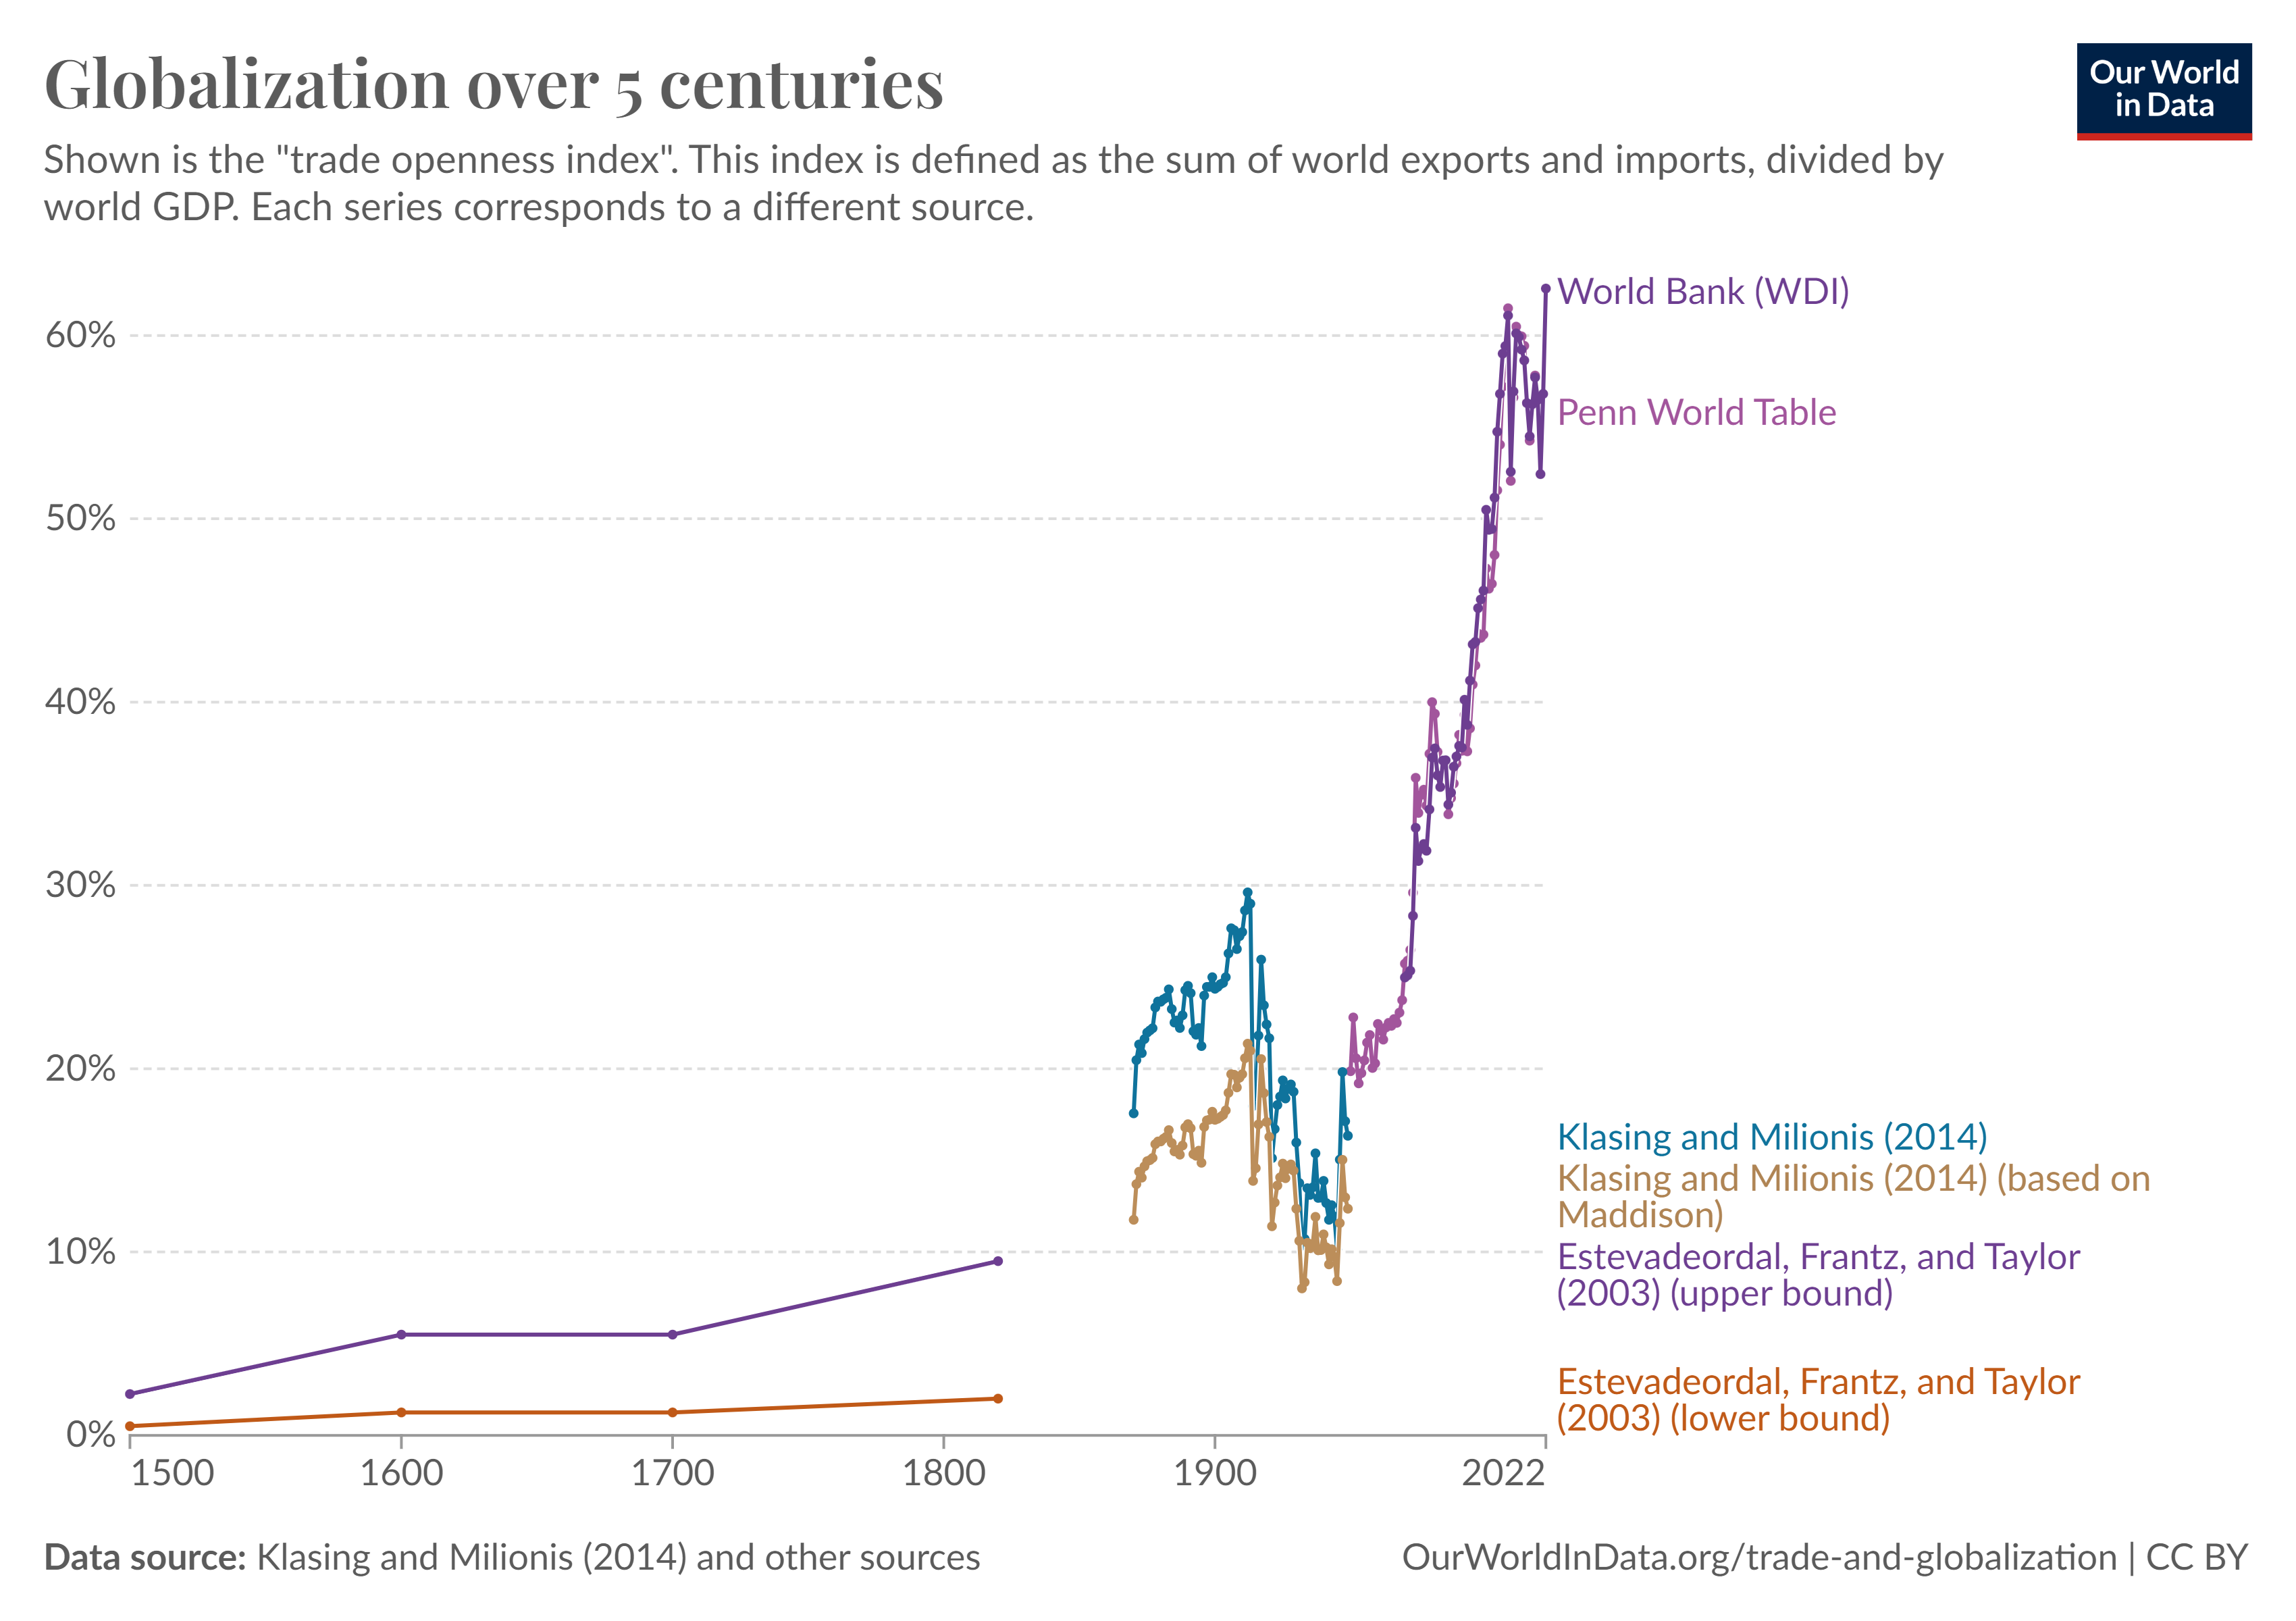
\includegraphics[scale=0.1]{globalization-over-5-centuries.png}
    \caption{Globalization over 5 centuries}
    \label{fig:globalizationOver5Centuries}
    \citep{ourWorldInData2023globalization5centuries}
\end{figure}

The concept of globalization encompasses various dimensions, including economic, political, cultural, and technological, each of which contributes to the deepening of global connections. Theoretically, globalization is driven by several factors \citep{thompson2023factors}, including:
\begin{itemize}
    \item \textbf{Technological advancements:} Innovations in transportation and communication technologies have significantly reduced the costs of doing business across borders. The transport sector’s efficiency saw significant improvements with the advent of multimodal transport, which integrates maritime and surface transportation. This development enhanced connectivity within countries and with neighboring nations, facilitated by highways and roads. The rise of digital platforms and e-commerce has transformed how businesses operate and reach global markets. Instant communication and online transactions have made cross-border trade more accessible.
    \item \textbf{Reduced trade barriers:} Governments have lowered tariffs, quotas, and other trade restrictions, facilitating the flow of goods and services between countries. The reduction of trade barriers, such as tariffs and quotas, has facilitated the free flow of goods and services across borders. This has been supported by international trade agreements and organizations.
    \item \textbf{The rise of multinational corporations:} Businesses with operations in multiple countries have played a crucial role in driving globalization by investing in foreign markets and economies of scale.
    \item \textbf{Financial liberalization:} Deregulation of financial markets has allowed for the free movement of capital across borders, promoting cross-border investments and trade.
\end{itemize}

\section{Economic Inequality}\label{economicInequality}

Economic inequality refers to the unequal distribution of income and wealth within and between populations. It can manifest in various forms, including income inequality, wealth inequality, and disparities in access to education, healthcare, and opportunities. Economic inequality is typically measured using indices such as the Gini coefficient, which quantifies the degree of inequality on a scale from 0 (perfect equality) to 1 (maximum inequality) (Deininger \& Squire, 1996).

Theoretical perspectives on economic inequality have evolved over time. Classical economists like Adam Smith and David Ricardo acknowledged the existence of inequality but emphasized the role of free markets in promoting efficiency and growth. In contrast, Marxist theories highlighted the exploitative nature of capitalism, where wealth accumulates in the hands of a few, leading to systemic inequality (Marx, 1867). More recent theories, such as those proposed by Piketty (2014), suggest that the dynamics of capital accumulation in a globalized economy tend to exacerbate inequality, as returns on capital often outpace economic growth.


\section{Globalization and Economic Inequality}\label{globalizationEconomicInequality}

Economic development has benefited from increased globalization, but this has also come at the cost of greater income inequality between countries.
The relationship between globalization and income inequality is a complex and 
multifaceted issue that has attracted considerable attention from scholars, policymakers, and the general public. As economies become more integrated into the global system, questions arise about the distributional consequences of this process. The overarching aim of this research paper is to conduct a comprehensive analysis of the impact of globalization on income inequality, delving into the nuanced dynamics that underlie this relationship.
Historically, the discourse surrounding globalization and income inequality has been polarized, with divergent views on the extent and nature of their correlation. Some argue that globalization fosters economic growth, leading to a rise in overall income levels and, consequently, a reduction in poverty. Conversely, critics contend that globalization exacerbates income inequality by favoring certain segments of the population, often those with access to capital and skills, while leaving others behind.


\chapter{Globalization and Economic Inequality: A Literature Review} \label{chapter:literatureReview}
\textit{This chapter is divided into three main sections. The first section addresses in detail the development of Autonomous Vehicle Technology and its impact in the mobility sector. The second section discusses the concept of Shared Autonomous Mobility (SAM) and the literature on the conception of carsharing methods and the shared economy and in the latter part of this section; the shared autonomous mobility services and the corresponding models from different studies are discussed. The final section addresses the fleet management and dynamic scheduling concepts. An overview of the various fleet management problems discussed in different studies along with the solution methodologies adopted till today (for the SAV services as well), is provided.}


. The advanced driver assistance technologies that it uses include a combination of sensor technologies for detecting and perceiving the environment around the vehicle followed by sending information to the driver and taking actions when required. The different types of ADAS sensors used in the autonomous vehicles in the market today is depicted in the figure below \citep{2021whatisadas}. An ADAS-equipped vehicle consisting of a group of these advanced multi-function sensors that provide output to the driver can primarily enhance the safety of vehicles and the environment and greatly reduce the human error factor.
% \begin{figure}[H]
%   \centering
%     \includegraphics[scale=0.3]{Inserts/figures/adas-sensors.jpg}
%     \caption{Diiferent types of ADAS sensors in Autonomous Vehicles \citep{2021whatisadas}}
%     \label{fig: adas sensors}
% \end{figure}


\chapter{Trend Analysis: Globalization and Economic Inequality in Developed and Developing Countries}\label{chapter:trendsAnalysis}
\chapter{Case Studies: Selected Countries} \label{caseStudies}
\chapter{Conclusion and Discussion}\label{chapter:conclusion&discussion}
The Shared Autonomous Mobility (SAM) concept overall has gained a significant positive reputation in many researches and studies, with autonomous shuttles having the potential to mitigate a good number of the existing problems related to traffic, environmental, overall costs incurred, last mile transportation, service fares, etc. that exist with the public transportation today and which have made it unfavourable for an average daily commuter to not opt for a privately owned car. The HEAT (Hamburg Electric Autonomous Transportation) research and development project is a pilot in HafenCity, Hamburg which tests the autonomous shuttle system in an urban environment and aims for the integration of an autonomous minibus (shuttle) service into the regular traffic of HafenCity. With a high focus on safety and operational capabilities, its efficient implementation on HafenCity network demonstrates the positive effects that innovative and ingenious mobility concepts can have in overcoming the limitations of the existing framework.

This thesis focused on the traffic and pedestrian simulation-based analysis through an agent based modeling of the operational requirements of the HEAT autonomous shuttles for a special-event scenario in HafenCity. Taking the scenario of a concert event at the \textit{Elbphilharmonie}, the idea was to check the efficiency and provide solutions for the HEAT autonomous shuttle operation, as a public transport, in providing service to the influx of pedestrians that enter the HafenCity network who, after the event has ended, are coming out from the venue, for a two hour period, i.e., from 18:00 to 20:00 hours. For this purpose, a microsimulation model for the entire HafenCity road network was developed and the public transport services, modeled for autonomous vehicle operation, was included, using the Aimsun Next software. A pedestrian area with one pedestrian entrance (Elbphilharmonie) and three different pedestrian exits were defined in the model through which all the pedestrians would enter and wait for the shuttle service at the PT stop; and finally exit the network after they alight from the vehicle. For this thesis, two primary indicators for measuring the pedestrian demand were selected with respect to Aimsun Next, namely, the \textit{Pedestrian Waiting Time at PT Stop} and the \textit{Pedestrian Travel Time}.

Keeping in mind the objectives of this study, five main scenarios were drawn and evaluated based on the two parameters for the implementation of methodology. The results were tabulated and plots were drawn for each parameter values in all the scenarios. The first two scenarios dealt with the initial existing cases of situation when the PT operates with time interval between departures at 10 minutes (\ref{scenario1}) and 5 minutes (\ref{scenario2}).The unreasonable and incredibly high average values of waiting time at PT stop (17.97 minutes and 15.14 minutes, respectively) and overall travel time (38.86 minutes and 23.39 minutes, respectively) values showed the insufficiency in the current service for the pedestrian demand. From careful examination of the results and plots, a \textit{peak hour} period was identified for which the cumulative increase in the demand values were impractical, which was found to be from 19:00 to 20:00 hours. This brought the focus on looking at this as a dynamic scheduling at the peak hour problem and attempting to solve for this through the implementation of certain functions from the Aimsun Next API module through direct programming (in this study, Python). Functions for dynamically changing mainly three different properties or factors influencing the public transport operation were investigated. While there was a direct function available for changing the maximum desired speed (from 15 km/h to 25 km/h) and modifying the PT vehicle route in such a way that the PT stop which was not utilized by the pedestrians to board or alight from the bus is skipped (the \textit{"Am Sandtorkai"} bus stop in the network) during the peak hour (\ref{scenario3}), a direct function could not be found for changing/influencing the schedule or timetable of the PT vehicle route. However, a workaround for solving for this issue was found which involved a case when the vehicle operates on the route with the time interval between departures at 5 minutes as usual and during the peak hour, an additional vehicle is introduced in the network using Aimsun API module with time interval between departures at every 3 minutes on the route. (\ref{scenario4}).

For the case of \ref{scenario3}, the results showed a considerable but not sufficient decrease in the pedestrian waiting time (11.17 minutes) and the overall pedestrian travel time (18.76 minutes). The relatively improved results also showcased that the approach of implementing API functions during the peak hour could be a considerable one for this study. This became evident when the results for \ref{scenario4} were examined. When compared to existing scenarios (\ref{scenario1} and \ref{scenario2}), it was observed that the pedestrian demand decreases by a large extent with the pedestrian waiting time and the overall travel time values (7.67 minutes and 15.84 minutes, respectively) reducing by more than 50\%. The final scenario (\ref{scenario5}) considered the case of combining the scenarios 3 and 4 (in sections \ref{scenario3} and \ref{scenario4} respectively). The results and their plots for the pedestrian waiting times (5.25 minutes) and overall travel times (11.98 minutes) show, upon proper implementation, a compelling use case of the HEAT autonomous shuttle service as a user-oriented public transportation even in a worst case (special-event) scenario of pedestrian demand peaks the network of HafenCity, such as the one considered in this thesis study, and beyond. A possible direction for further research and related studies in the future could be conducting an operational fleet management study of deployment of autonomous shuttles which is based on the pedestrian requests making it a truly demand-responsive request based system.

Therefore, it can also be understood that a carefully planned and efficiently managed fleet of the user-oriented shared autonomous vehicles (such as the HEAT autonomous shuttles), when shifted from the pilot stage and brought to the urban areas as a feeder service with proper implementation depending on the urban environments and population, have the potential to bring reforms and ameliorate the public transportation systems of the future along with shaping the way urban mobility is seen today.





\printbibliography{}


\clearpage


% \begin{appendices}
% \appendix
% \input{pages/appendix}
% \end{appendices}
% %\appendix
%  %\renewcommand*\printchaptername{\Large\bfseries\appendixname~}




\microtypesetup{protrusion=false}
\microtypesetup{protrusion=true}


\end{document}
